\documentclass{article}
\usepackage{booktabs}
\usepackage[margin=1in]{geometry}
\usepackage{amsmath}
\usepackage{amssymb}
\usepackage{graphicx}
\usepackage{caption}

\newcommand{\ra}[1]{
\renewcommand{\arraystretch}{#1}}
\newcommand{\pa}[1]{\noindent\textbf{\textsf{#1}}}
\newcommand{\x}{\mathbf{x}}
\newcommand{\demand}{\mathbf{d}}
\newcommand{\y}{\mathbf{y}}
\newcommand{\w}{\mathbf{w}}
\newcommand{\s}{\mathbf{s}}
\newcommand{\A}{\mathbf{A}}


\title{\textsf{Multi-Echelon Inventory Control for Perishable Products}}
\author{\textsf{}}
\date{\textsf{\today}}

\begin{document}

\maketitle

\pa{Model Setup}
\begin{itemize}
	\item Total $T$ time periods. 
	\item Network with incidence matrix $A$.
	\item Single product, life time is $m$.
	\item Lead times are fixed ($l_{ij}$).
	\item There are yield and storage capacities.
	\item Sequence of events:
	\begin{enumerate}
		\item Demand realization
		\item Allocation of inventories to demand
		\item Disposal and expiration
		\item Previous orders arrive
		\item Inventory state update
		\item Place order
	\end{enumerate}
	\item Decisions include inventory attribution, disposal, and ordering.
	\begin{itemize}
	\item Why not FIFO? Maximizing freshness might require non-FIFO.
	\item Why disposal? Disposal makes sense when we have storage capacity.
	\end{itemize}
\end{itemize}


\section*{Single Node Single Source}

Assumptions
\begin{itemize}
\item Lead time $l$, same freshness ($m$ remaining) when arriving
\end{itemize}

\begin{table*}[h!]
\centering
\ra{1.3}
\begin{tabular}{@{}cl@{}}
\toprule
Variable & Description \\
\midrule
$x_{k}$ & life-$k$ inventory in the beginning of period, $k=1,\dots,m+l$\\
$y$ & order quantity in the beginning of the period \\
$w_{k}$ & wastage of life-$k$ inventory after demand realization in $t$ \\ 
$s_{k}$ & demand satisfaction with life-$k$ after demand realization \\
$d$ & demand\\
$\bar{x}$ & storage capacity at retailer \\
$\bar{y}$ & ordering capacity per period \\
\bottomrule
\end{tabular}
\end{table*}

Minimizing wastage: $$J^t(\x^t) = \min_{y \geq 0} \max_{d^t \in U^t} \; \min_{(\s^t,\w^t) \in V^t(d,y,\x)}  \; \mathbf{1}' \w^t + J^{t+1}(f(\x^t, \w^t, \s^t, y))$$
where the feasible region $V^t(d,y,\x)$ is 
\begin{align*} 
   \sum_{k \in [m]} s_{k}^t \geq d^t && \forall d^t \in U^t && \text{(demand satisfaction)} \\
   s_{k}^t + w_{k}^t \leq x_{k}^t && \forall k \in [m] && \text{(inventory allocation)} \\
   w_{1}^t = x_{1}^t && && \text{(expiration)} \\
   y^t \leq \bar{y}^t && && \text{(yield capacity)} \\
   %\sum_{k \in [m]} y^{t}_{ijk} \leq u_{ij}^t && \forall (i,j) \in A && \text{(transportation capacity)} \\
   \sum_{k \in [m]} x^t_{k} \leq \bar{x}^t &&  && \text{(storage capacity)}
\end{align*}

And the linear update rule is $$f_k(\x,\w,\s,y) := x_{k+1} - w_{k} - s_{k}, \quad k=1,\dots,m+l-1,$$
$$f_m(\x,\w,\s,y) = y.$$

Last time period: $$J^T(\x^T) = \min_{y \geq 0} \max_{d^T \in U^T} \; \min_{(\s^T,\w^T) \in V^T(d,y,\x)}  \; \mathbf{1}' \w^T ,$$
where $V^T(d,y,\x)$ is described by:
\begin{align*} 
   \sum_{k \in [m]} s_{k}^T \geq d^T && \forall d^T \in U^T && \text{(demand satisfaction)} \\
   s_{k}^T+ w_{k}^T \leq x_{k}^T && \forall k \in [m] && \text{(inventory allocation)} \\
   w_{1}^T = x_{1}^T && && \text{(expiration)} \\
   y^T \leq \bar{y}^T && && \text{(yield capacity)} \\
   \sum_{k \in [m]} x^T_{k} \leq \bar{x}^T &&  && \text{(storage capacity)}
\end{align*}
What value of $d^T$ does it take from $U^T$? If the problem is infeasible for some $d^T \in U^T$, then $d^T$ will always take such value (e.g., the largest) to take the cost to infinity. But assuming we have come to a point where feasibility is satisfied, then $d^T$ will actually take the smallest value. 

\section*{Single Node, Multisource}

\section*{Bipartite}

\pa{Variables \& Parameters}

\begin{table*}[ht]
\centering
\ra{1.3}
\begin{tabular}{@{}cl@{}}
\toprule
Variable & Description \\
\midrule
$x_{jk}^{tl}$ & life-$k$ in-transit inventory $l$ periods away from $j$ in the beginning of period $t$ \\
$x_{jk}^{t}$ & life-$k$ on-hand inventory at $j$ in the beginning of period $t$ \\
%& $x_{j1}^t,\dots, x_{jm}^t$ are on-hand inventories with life $1,\dots,m$ \\
%& $x_{j(m+1)}^t, \dots, x_{j(m+l)}^t$ are in-transit inventories, $l = \max_{i} l_i$ \\
$y_{ijk}^t$ & order quantity of life-$k$ product from $i$ to $j$ by the end of period $t$ \\
%& $y_{ij}^t$ is added to $x^t_{j(m+)}$ \\
$w_{jk}^t$ & wastage of life-$k$ inventory after demand realization in $t$ \\ 
$s_{jk}^t$ & demand satisfaction with life-$k$ after demand realization in $t$ \\
$d_j^t$ & demand in node $j$ in period $t$ \\
\bottomrule
\end{tabular}
\end{table*}

\pa{Formulation}
\newline

Minimizing wastage: $$J^t(\x^t) = \min_{(\s^t,\w^t,\y^t) \in V^t}  \; \mathbb{E} \left[\mathbf{1}' \w^t + J^{t+1}(f(\x^t, \w^t, \s^t, \y^t)) \right] $$

Maximizing freshness: $$J^t(\x^t) = \max_{(\s^t,\w^t,\y^t) \in V^t} \; \mathbb{E} \left[\sum_{j \in J} \sum_{k \in [m]} k s_{jk}^t / (md_j^t) + J^{t+1}(f(\x^t, \w^t, \s^t, \y^t))\right]$$


where the feasible set for controls in period $t$ is:

\begin{align*} 
   \sum_{k \in [m]} s_{jk}^t \geq {\delta} d_j^t && \forall j \in J && \text{(demand satisfaction)} \\
   s_{jk}^t + w_{jk}^t \leq x_{jk}^t && \forall j \in J, k \in [m] && \text{(inventory allocation)} \\
   w_{j0}^t = x_{j0}^t && \forall j \in J && \text{(expiration)} \\
   %\sum_{j \in J} y^t_{ijk} \leq \bar{y}^t_{ik} && \forall i \in I, k \in [m] && \text{(yield capacity)} \\
   %\sum_{k \in [m]} y^{t}_{ijk} \leq u_{ij}^t && \forall (i,j) \in A && \text{(transportation capacity)} \\
   %\sum_{k \in [m]} x^t_{jk} \leq \bar{x}_j^t && \forall j \in J && \text{(storage capacity)}
\end{align*}
The linear update rule $f(\cdot)$ is a vector-valued function, dependent on the lead times and orders from upstream nodes: $$x^t_{jk} = x^{(t-1)1}_{j(k+1)} + x^{t-1}_{j(k+1)} - s^{t-1}_{j(k+1)} - w^{t-1}_{j(k+1)},$$
$$x^{tl}_{jk} = x^{(t-1)(l+1)}_{j(k+1)} + \sum_{i : l_{ij} = l} y^{t}_{ijk}$$
\newline

\pa{Notes}
\begin{itemize}
\item Decomposable across $j$ if relax yield capacity constraint.
\item Reduce the state space and decision space if we are minimizing expiration instead of maximizing freshness: do not have to keep track of the shelf life of inventory arriving from supplier.
\item Would maximizing freshness lead to ordering a lot and just serving demands with freshest inventory?
\end{itemize}


\pa{Single Node Uncapacitated Policy}
\newline 

Chen, Pang, and Pan (2014) setup:
\begin{itemize}
\item lead time is $k$
\item product life is $l > k$
\item FIFO policy
\item Ordering cost: $c$/unit, inventory cost $h^+$ and $h^-$, disposal cost $\theta$
\item Demand $d_t := D(p) + \epsilon_t$, where 
	\begin{itemize}
	\item $D(p)$ is strictly decreasing
	\item $\epsilon_i$ is i.i.d., zero mean, with bounded support $[A,B]$ 
	\item Price is bounded $[\underline{p}, \bar{p}]$
	\end{itemize}
\item Decisions: ordering, pricing, disposal. 
\end{itemize} 


\pa{Simplifications}

\begin{itemize}
\item Assume no storage capacity, then with low/zero inventory holding cost $\rightarrow$ FIFO.
\item No inventory holding cost $\rightarrow$ no disposal.
\end{itemize}

\pagebreak

\section*{\textsf{Meetings and Planning}}

\pa{June 27}

\begin{enumerate}
\item Include disposal and issuing decisions to keep the model open
\item If supplier capacitated by residual life, then need to keep supplier inventory vector and therefore do inventory update (add a constraint)
\item Would the current case lead to trivial solution that uses demand upperbound
\item Solve the formulation for one node for now, and check against the literature (Chen et al) to see if solution makes sense.
\item Whether expected value or robust problem easier? Explore policy structure or solve numerically?
\item Adaptive/adjustable robust 
\end{enumerate}

To address these questions, do the following steps by Friday:
\begin{itemize}
\item Formulate the one-node case (with and without capacity)
\item Comparison with existing models
\item Solution methods, difficulties
\end{itemize}


\pa{June 29 - Project Plan}

\begin{table*}[h!]
\small
\centering
\ra{1.3}
\begin{tabular}{@{}lccc@{}}
\toprule
Model Feature & Model 1 (July 6) & (July 13) & Model 2 (Aug 10) \\
\midrule
Network & Single node multi-source & -- & Multi-echelon \\
Objective & $\max \; \mathbb{E}$[freshness - waste - demand loss] & Sensitivity & -- \\
Capacity & Exogenous capacity & -- & Outflow capacitated by inv \\
Inventory Issuing & FIFO & -- & (Active issuing) \\
Disposal Policy & Expiration only & -- & (Active disposal) \\
Coordination & Centralized decision & -- & (Distributed vs. Centralized) \\
Solution Approach & Heuristic & Implementation & (Bounds and Theory) \\
\bottomrule
\end{tabular}
\end{table*}

Model 1 deviates from the literature mostly on the multi-sourcing aspect. This introduces modeling and computational challenge since we need to introduce an additional dimension when tracking inventory. Model 2 expands to multi-echelon network. Tasks in brackets have lower priority for now.

Model 1: For each period, we use $x_{kl}$ to denote the amount of inventory with $k$ periods left in shelf life, which we have held for $l$ periods. For $l < 0$, the inventory is arriving in $|l|$ periods. Thus when we order from supplier $i$ with lead time $L_i$, we update the vector $x_{1L_i},\dots,x_{mL_i}$. For $l > 0$, we are keeping track of how long we have held the inventory in our current location, which allows us to calculate freshness (both for inventory freshness and demand satisfaction freshness). 

Model 2: When extending to multi-echelon, we update the supply capacity by the upstream inventory levels, which are subject to state transition.
\newline

Comments from the June 29 meeting:

\begin{itemize}
\item For model 1, assume single bucket of age and lead time (different each source of course).
\item For implementation: 3 tiers including farms, suppliers, and retailers.
\item Include a service level constraint, and then penalize the loss demand beyond that.
\item System performance comparison (on a simulator)
	\begin{itemize}
	\item Base stock policy, order from closest supplier/farm. [Key]
	\item Single-echelon-optimal-policy at last tier (tier $n$), and base stock everywhere else. 
	\item Single-echelon-optimal-policy everywhere, empirical demand signal at $i$ from 1 tier down $\mathbb{P}[D_{i+1}]$.
	\item Single-echelon-optimal-policy everywhere, demand signal visible $\mathbb{P}[D_{n}]$, and know $\mathbb{P}[D_i | D_n]$. [blockchain visibility]
	\item Multi-echelon centralized decision [blockchain coordination]
	\end{itemize}
\item Build the simulator.
\end{itemize}


\pa{Aug 1 - Value of Visibility.}
\newline

\begin{enumerate}
\item Issuing policy: we find that in the farm-supplier-retailer chain, if farm issues ages $m$ and $m-1$ (50/50), vs. is better than issuing age $m-1$ and $m-2$ (50/50). This is a very specific made-up example (not sure what decision mechanism will lead to these numbers), but this shows the importance of (downstream lead time aware) issuing policy.
\item  Value of centralization must be strictly better than the value of visibility (with decentralized operations). So if we can quantify the value of centralization, we can upper bound the value of decentralized and visible operations. But the centralized case should be easy to implement for at least the base stock policy for a chain -- just assume the whole chain as a single echelon. To achieve this centralization, the information to be shared is just the lead times at every echelon, and the total inventory at each node. This looks trivial. Am I missing something?
\item To extend the intuition from chain to network, look at Cachon and Fisher (2000) since they considered a hub and spoke system.
\item Literature review: Cachon on supply chain contract. Other papers on (two-echelon) supply chain information sharing.
\end{enumerate}

% Python code is in the github version for Aug 1
\begin{minipage}[c]{0.5\linewidth}
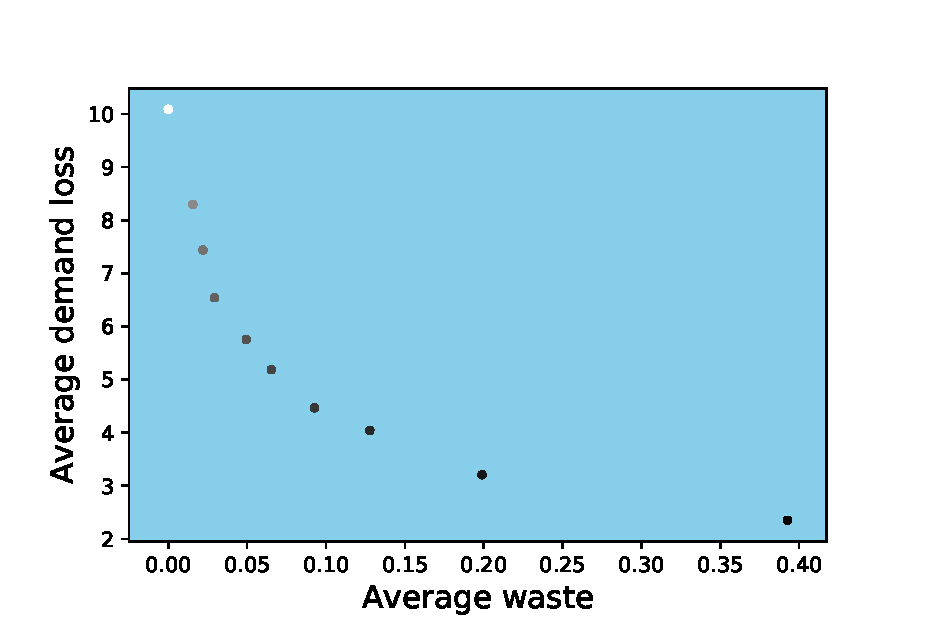
\includegraphics[width=\linewidth, trim=15 15 15 15, clip]{figures/demandLoss_vs_waste_decentralized.eps}
\captionof{figure}{Decentralized base stock policies.}
\end{minipage}
\begin{minipage}[c]{0.5\linewidth}
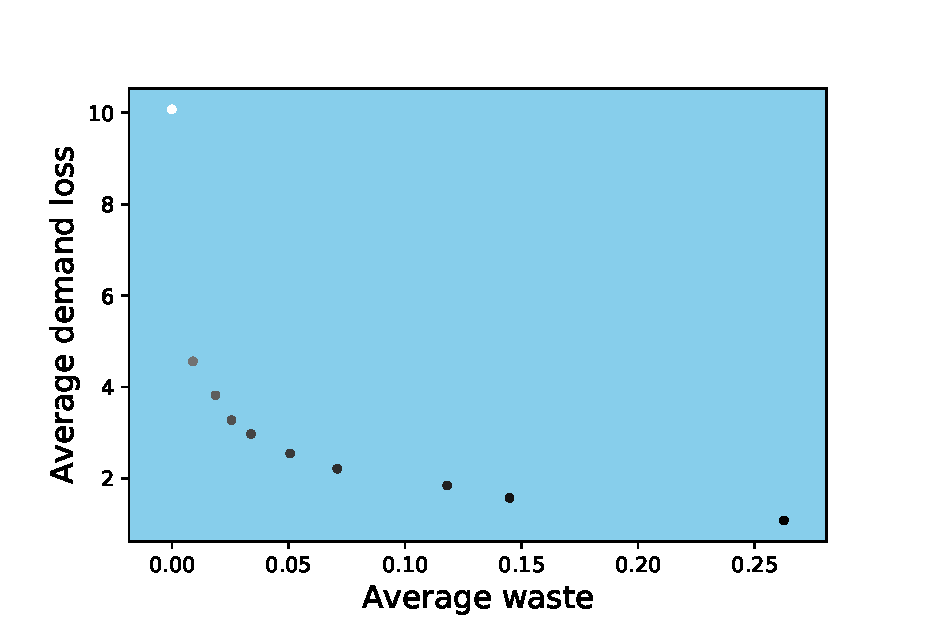
\includegraphics[width=\linewidth, trim=15 15 15 15, clip]{figures/demandLoss_vs_waste_centralized.eps}
\captionof{figure}{Centralized base stock policies.}
\end{minipage}
\newline
\newline

\pa{Aug 6 - Blockchain governance.}
\newline

Goal for the next three weeks: literature review of supply chain contract, blockchain, and blockchain application in the contracts.

At least two ways that blockchain contributes. Both ways are basically having the blockchain act as a game designer.
\begin{enumerate}
\item Blockchain can limit the space of actions (my thought).
\item Blockchain can change the types of contract from bilateral to multi-lateral (Ramesh).
\end{enumerate}

\pa{Aug 7 - Supply chain contracts day 1: newsvendor model.}

\begin{itemize}
\item Negotiation and blockchain: supply chain contract literature does not focus on the negotiation process. But in practice, this is a costly multi-period problem. Can blockchain provide anything here?
\end{itemize}

\pa{Aug 8 - Incentive for data sharing.}
\begin{itemize}
\item With blockchain, incentive is not about whether truthfulness of data, but about the revelation of data. 
\item Valuation of data: Munther's paper and Shapley value. For data duplication problems, check the dimensionality of the data.
\item Privacy: zero-knowledge proof.
\end{itemize}

\pa{Aug 9 - Vishal Gaur talk: the case of blockchain in supply chain management.}

\begin{itemize}
\item Three flows: physical, financial, and document. Physical flow not as well tracked as financial flow. The flows are usually disconnected. Do audits afterwards, but is post factor and expensive. 
\item Difference between scm and bitcoin: (1) anonymity not good for sc transactions. (2) Majority based distributed consensus not necessary for sc. Byzantine. (3) Both financial and non-financial data should be posted for sc. (4) Smart contracts, IoT, and distributed apps become far more useful in sc. (5) digitization of physical assets such inv and capacities. (6) Blockchain not designed for fast storage and retrieval, not good for certain type of actions (slow is related to the majority based distributed consensus). 
\end{itemize}

I feel that the key is data privacy in sharing onto a distributed ledger. Because like we thought about at the lunch meeting with Ashish and Pavithra, the key incentive question in these applications is not truthfully reporting data, but revealing certain data at all. Because untruthful reporting is now a documented fraud in blockchain. So the incentive problem changed. Furthermore, I think that if we focus on the soft (economic) incentive of sharing data at all, we have to work with specific problem instances, because this thing is highly sensitive to problem setup and blockchain implementation (?). Now think about 










\end{document}